\documentclass{article}
\usepackage[margin=.75in]{geometry}
\usepackage{graphicx, dblfloatfix}
\usepackage{amsmath, amssymb, amsfonts}
\usepackage[english]{babel}
\usepackage[autostyle, english = american]{csquotes}
\MakeOuterQuote{"}

\newenvironment{tightcenter}{%
  \setlength\topsep{0pt}
  \setlength\parskip{0pt}
  \begin{center}
}{%
  \end{center}
}

\newcommand{\redchi}{$\tilde{\chi}^2\,$}
\DeclareMathOperator\erf{erf}
\DeclareMathOperator\cov{cov}

\title{Gamma Cross Sections}
\author{Aman LaChapelle}

\begin{document}
\maketitle

	\begin{abstract}
		We measure the linear attenuation coefficient (as a function of photon energy) of Aluminum by using Ba-133 and Na-22 sources to produce gamma excitations at a range of energies, and measuring the excitations opposite Aluminum blocks of varying thickness.  We fit the countrates as a function of thickness of the Aluminum in order to find the Linear Attenuation Coefficient, $\lambda$.
	\end{abstract}


\tableofcontents
\newpage

\section{Introduction}
	Photons incident on matter will cause a number of reactions depending on their energy.  As seen in Figure 1, the low energy photon interactions will be governed largely by the photo-electric effect.  At slightly higher energies, (approx. $0.2 \, MeV$ - approx. $5 \, MeV$) the interactions will be governed by Compton Scattering.  At higher energies still, ($>5 \, MeV$) the interactions will be governed by pair production of a photon into an electron and a positron.  We will use fits of the PHA cross sections to find the counts of photons at each energy under test.  We will use those counts to find countrates, and fit again to a decaying exponential to determine the linear attenuation coefficient, $\lambda$.
	
	\hspace{1cm}

	\begin{figure}[!htb]
		\centering
		\includegraphics[scale=.25]{linear_attenuation_coefficient_al}
		\caption{The figure continues to the right, we will begin to see pair production dominate as 
		the energy of the photon increases.  Shamelessly taken from the manual. \cite{lab manual}}
	\end{figure}

\section{Theory}
	If we have some material with free valence electrons we will have some density of electrons on the surface of the material equal to 
	\begin{equation}
		\sigma = N \times A_{e}
	\end{equation}
	with $N$ being the number of electrons on the surface, and $A_{e}$ being the average area per electron
	Given this expression for the surface density of electrons we can write the density of electrons in a 3-D substance as
	\begin{equation}
		\rho = \sigma d\ell
	\end{equation}
	with $d\ell$ being the depth of the material, assuming the electon density in each $d\ell$ is roughly the same.
	\hspace{.5cm}
	\begin{flushleft}
	With this expression for the electron density, we can find the reduction in intensity of a photon that passes through the material due to electron collision.  We write
	\end{flushleft}
	\begin{gather*}
		dR = -\rho R\\
		R(\ell) = e^{-\rho(\ell) + R_0} + C
	\end{gather*}
	using equation (2) to rewrite results, 
	\begin{gather*}
		R(\ell) = R_0e^{-\sigma \ell} + C\\
		R(\ell) = R_0e^{-\frac{\sigma}{\ell} \ell} + C\\
	\end{gather*}
	\begin{equation}
		\boxed{R(x) = R_0e^{-\lambda x} + C}
	\end{equation}
	We define $\lambda$, the linear attenuation constant, with units of per cm as $N \times A_{e}$.  We use $x$ here instead of $\ell$ suggestively to emphasize the fact that this will be used as the model to find $\lambda$ later on, and to bring to mind the cartesian plane.


\section{Apparatus}
	The apparatus consisted of a Ba-133 or Na-22 source approx 15.6 cm from a clear plexiglass plate fitted to hold the Aluminum disks we used.  We had disks of thickness 1mm, 2mm, 4mm, 8mm, 16mm and 32mm and used these and combinations thereof to get our data.  The source itself was approx 22.4 cm from the detector.

	\hspace{1cm}

	\begin{tightcenter}
	\begin{figure*}[!htb]
		\centering
		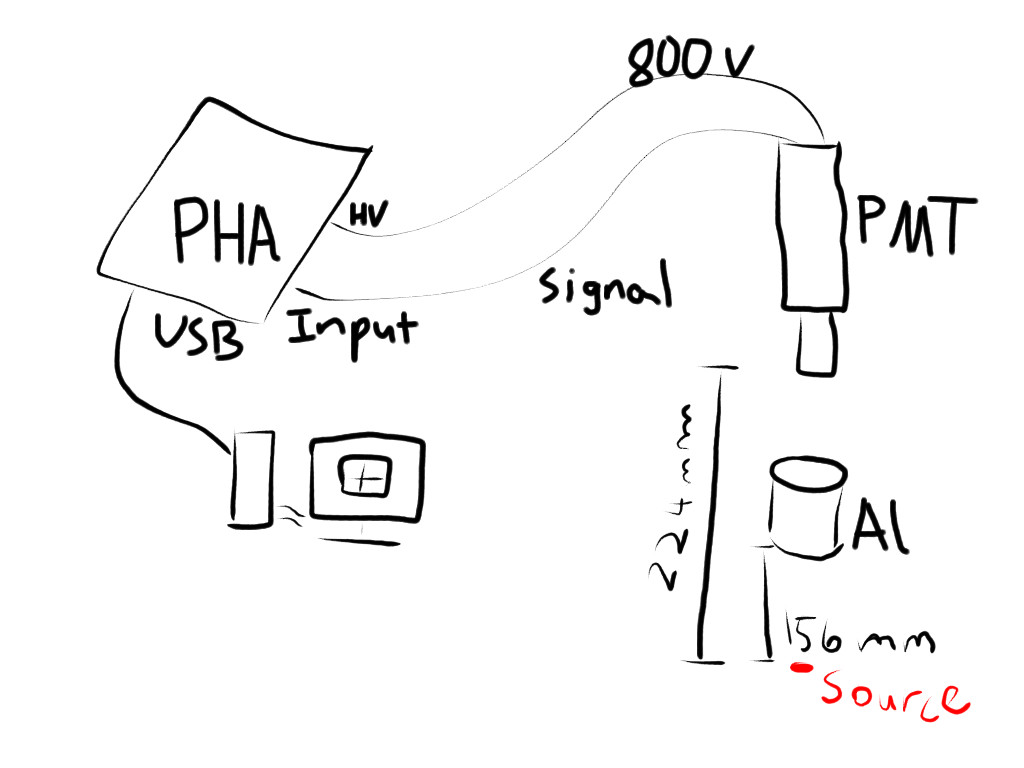
\includegraphics[scale=.3]{paint.jpg}
		\caption{Experimental Apparatus - note the distances marked in the figure, they make some small difference and caused some systematic uncertainty to enter into our data collection.}
	\end{figure*}
	\end{tightcenter}

	\begin{flushleft}
	Good geometry for the apparatus involves making sure that any photons that actually reach the detector come from the source that is directly below, and they must travel through the bulk of the aluminum and not scatter around the alumnum edge.  The photons especially must not scatter from elsewhere in the room, off the aluminum and into the detector.  Thus there is an optimal distance between the aluminum absorber and the detector that must be reached.  We experienced a systematic uncertainty, which we will discuss later that means our geometry was not perfect.  Nevertheless, we apply this systematic uncertainty to all our calculations beginning in the countrates.  It will be relevant to the number of counts and so we have added it to the uncertainty in the counts.  We add normally because if there is systematic uncertainty it is likely not independent of other uncertainty in the counts.  The systematic uncertainty we will add we estimate at 0.02 $cm^{-1}$, based on our final results.

	\vspace{.25cm}
	
	The apparatus consisted of a Photo Multiplier Tube connected via high voltage (800 V) to a Pulse Height Analyzer.  The PMT returns pulses of varying voltages to the PHA, which uses that voltage to decide where to bin the pulse data.  This is the step that introduces width to the gaussian shape of the pulse, we would expect that the photons would have a definite energy and thus in a perfect world we would fit to delta functions.  However, there will be noise in the lines, as well as a finite conductivity that causes broadening of the spectrum.  This is known as the absorber's resolution.
	\end{flushleft}
\section{Data Analysis}
	\subsection{PHA Cross Sections}
		The cross sections of the Pulse Height Analyzer (PHA) spectrum are what we see during data collection.  By selecting an Region of Interest (ROI) on the data collection software, the USX software could return to the user the net counts received by the Photo Multiplier Tube (PMT) by taking total counts within the ROI and subtracting the background using points at the edge of the ROI and subtracting points underneath that threshold.

		\begin{flushleft}
		We decided that the ROI settings were not consistent enough to properly minimize our error, and so we decided to use Gaussian fits to the data and use the amplitude as the net counts.  We fit to the function
		\end{flushleft}
		\begin{equation}
			f(x) = \frac{N}{\sigma\sqrt{2\pi}}e^{\frac{-(x-\mu)^2}{2\sigma^2}} + Ax + B
		\end{equation}
		as seen in Figures 3 and 4.  An important note about the uncertainties in the fit: the net counts are recorded as $N \pm \delta N = 7596 \pm 200$ counts, which is equivalent to $7596$ counts $\pm \, 2.6\%$ - a very small error overall, which is even smaller for larger values of $N$ as one might expect.

		\begin{flushleft}
		One important question to answer is why we would fit to a gaussian shape and not, say, a Lorentzian
		\end{flushleft}
		\begin{equation*}
			L(x) = \frac{1}{\pi} \frac{\frac{1}{2}\Gamma}{(x-x_0)^2 + \frac{1}{2}\Gamma^2}
		\end{equation*}
		which would also fit the data?  The answer comes from the assumption that the error comes from the detector apparatus.  Essentially, because the error (what gives width to the gaussian) is a counting error, which means that it acts on $\bar{x}$ as $\sigma_{\bar{x}}$, giving us a Gaussian distribution as we see in equation (4).

		\begin{flushleft}
		We take the values of the countrates calculated from the cross section fits and tabulate them here.  Values for Ba-133 are followed by values for Na-22.  Note the arbitrary precision - this is simply to avoid rounding error as we proceed forward.  The rules of significant figures and error propagation will be applied at the end.
		\end{flushleft}

		\begin{center}
		Ba-133 Countrates and Uncertainty\\
		\begin{tabular}{|l|l|l|l|l|l|l|}
			\hline
			Thickness (mm) & N1 (count/s) & N2 (count/s) & N3 (count/s) & $\delta$N1 & $\delta$N2 & $\delta$N3\\ \hline \hline
			56 & 9.044 & 9.910 & 39.361 & 1.915\% & 4.832\% & 1.959\%\\ \hline
			40 & 13.480 & 20.943 & 57.620 & 2.632\% & 3.389\% & 2.156\%\\ \hline
			32 & 16.963 & 29.207 & 73.845 & 1.895\% & 1.467\% & 1.451\%\\ \hline
			16 & 29.924 & 77.124 & 110.873 & 1.755\% & 1.021\% & 1.658\%\\ \hline
			8 & 80.258 & 111.341 & 136.650 & 1.520\% & 1.461\% & 2.083\%\\ \hline
			4 & 190.564 & 132.989 & 147.288 & 1.074\% & 1.026\% & 2.086\%\\ \hline
			2 & 303.314 & 145.682 & 156.056 & 1.094\% & 1.302\% & 2.127\%\\ \hline
			1 & 391.492 & 152.985 & 155.885 & 1.032\% & 1.320\% & 2.074\%\\
			\hline
		\end{tabular}
		\end{center}

		\begin{center}
		Na-22 Countrates and Uncertainty\\
		\begin{tabular}{|l|l|l|l|l|}
			\hline
			Thickness (mm) & N1 (count/s) & N2 (count/s) & $\delta$N1 & $\delta$N2\\ \hline \hline
			1 & 406.078 & 75.520 & 0.517\% & 1.359\%\\ \hline
			2 & 394.042 & 73.181 & 0.599\% & 1.360\%\\ \hline
			8 & 352.798 & 67.239 & 0.676\% & 1.425\%\\ \hline
			16 & 301.809 & 61.899 & 0.910\% & 1.545\%\\ \hline
			40 & 183.388 & 44.981 & 1.532\% & 1.901\%\\ \hline
			61 & 118.990 & 32.176 & 1.874\% & 2.226\%\\
			\hline
		\end{tabular}
		\end{center}

		\begin{tightcenter}
		\begin{figure}[!htb]
			\centering
			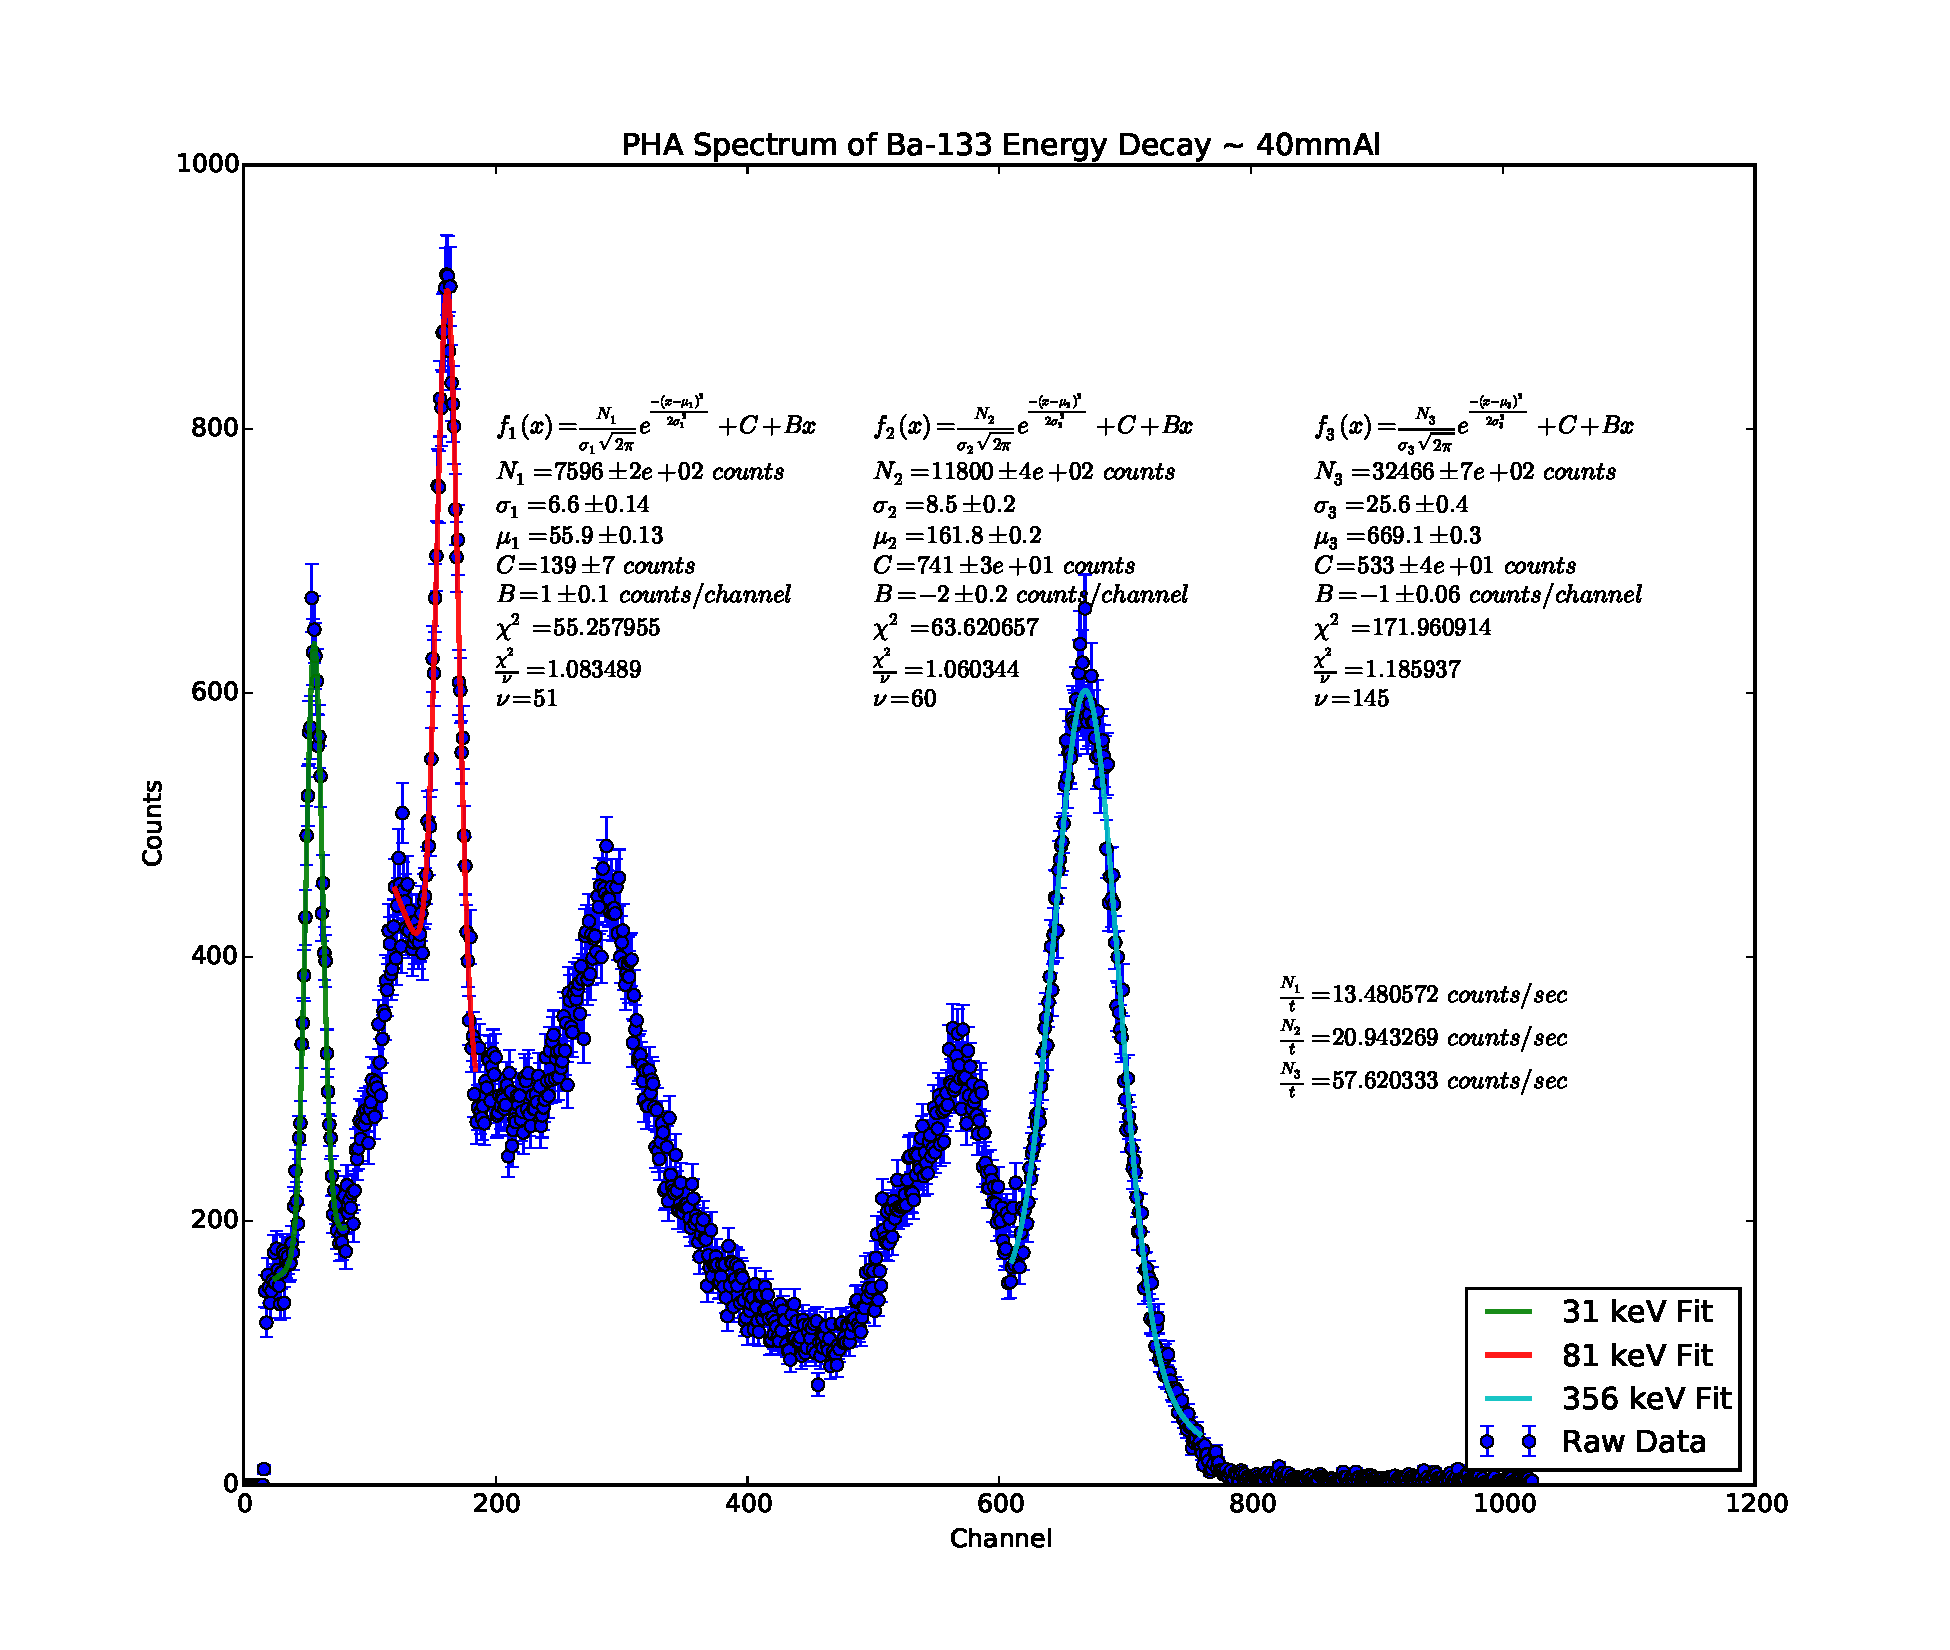
\includegraphics[width=13cm,height=7.5cm]{../plots/Ba40mmAl.pdf}
			\caption{A sample fit from a Ba-133 PHA spectrum, all three peaks of interest were fit to different gaussians and based on length (in time) of data collection, the count rates were calculated and added to the plot for reference.  The other peaks are the backscatter and compton features, more clearly seen and identified on the Na-22 plots.}
		\end{figure}

		\begin{figure}[!htb]
			\centering
			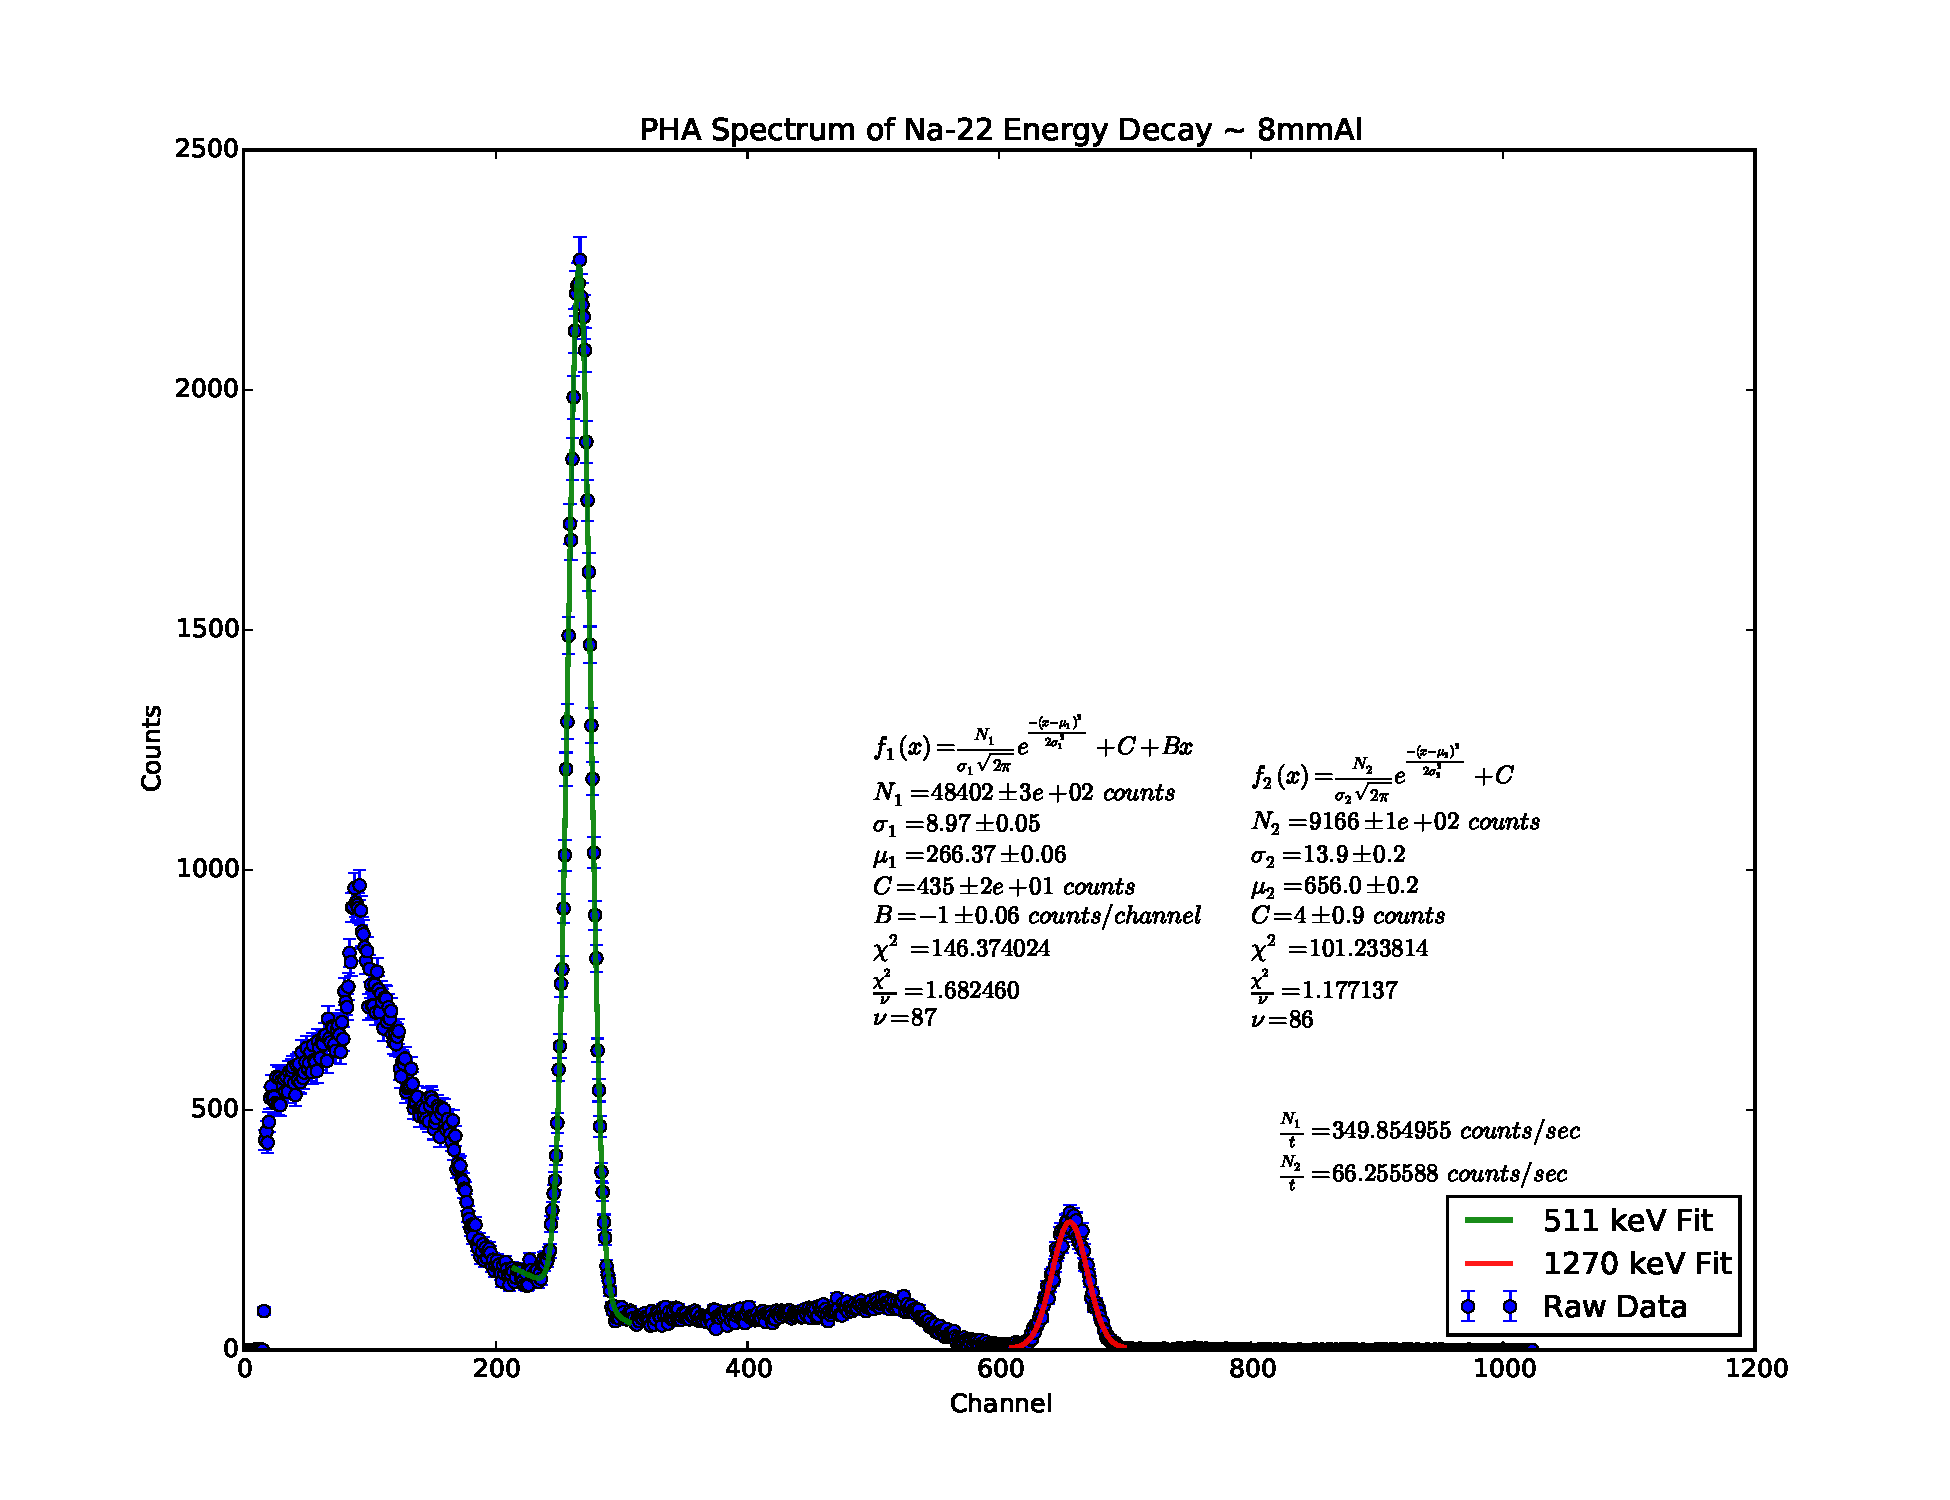
\includegraphics[width=11cm,height=7.5cm]{../plots/Na8mmAl.pdf}
			\caption{A sample fit from a Na-22 PHA spectrum, again the two peaks of interest were fit to separate gaussians.  The peak furthest to the left of the spectrum is the backscatter peak, and the plateau background it sits on is the compton shelf.  The declining edge that leads into the peak of interest is the compton edge.}
		\end{figure}
		\end{tightcenter}

	\subsection{Countrates}

	Using the data tabulated for the Na-22 and Ba-133 countrates we fit the exponential form found in equation (3).

	\subsubsection{Na Countrates}

	\begin{tightcenter}
	\begin{figure}[!htb]
		\centering
		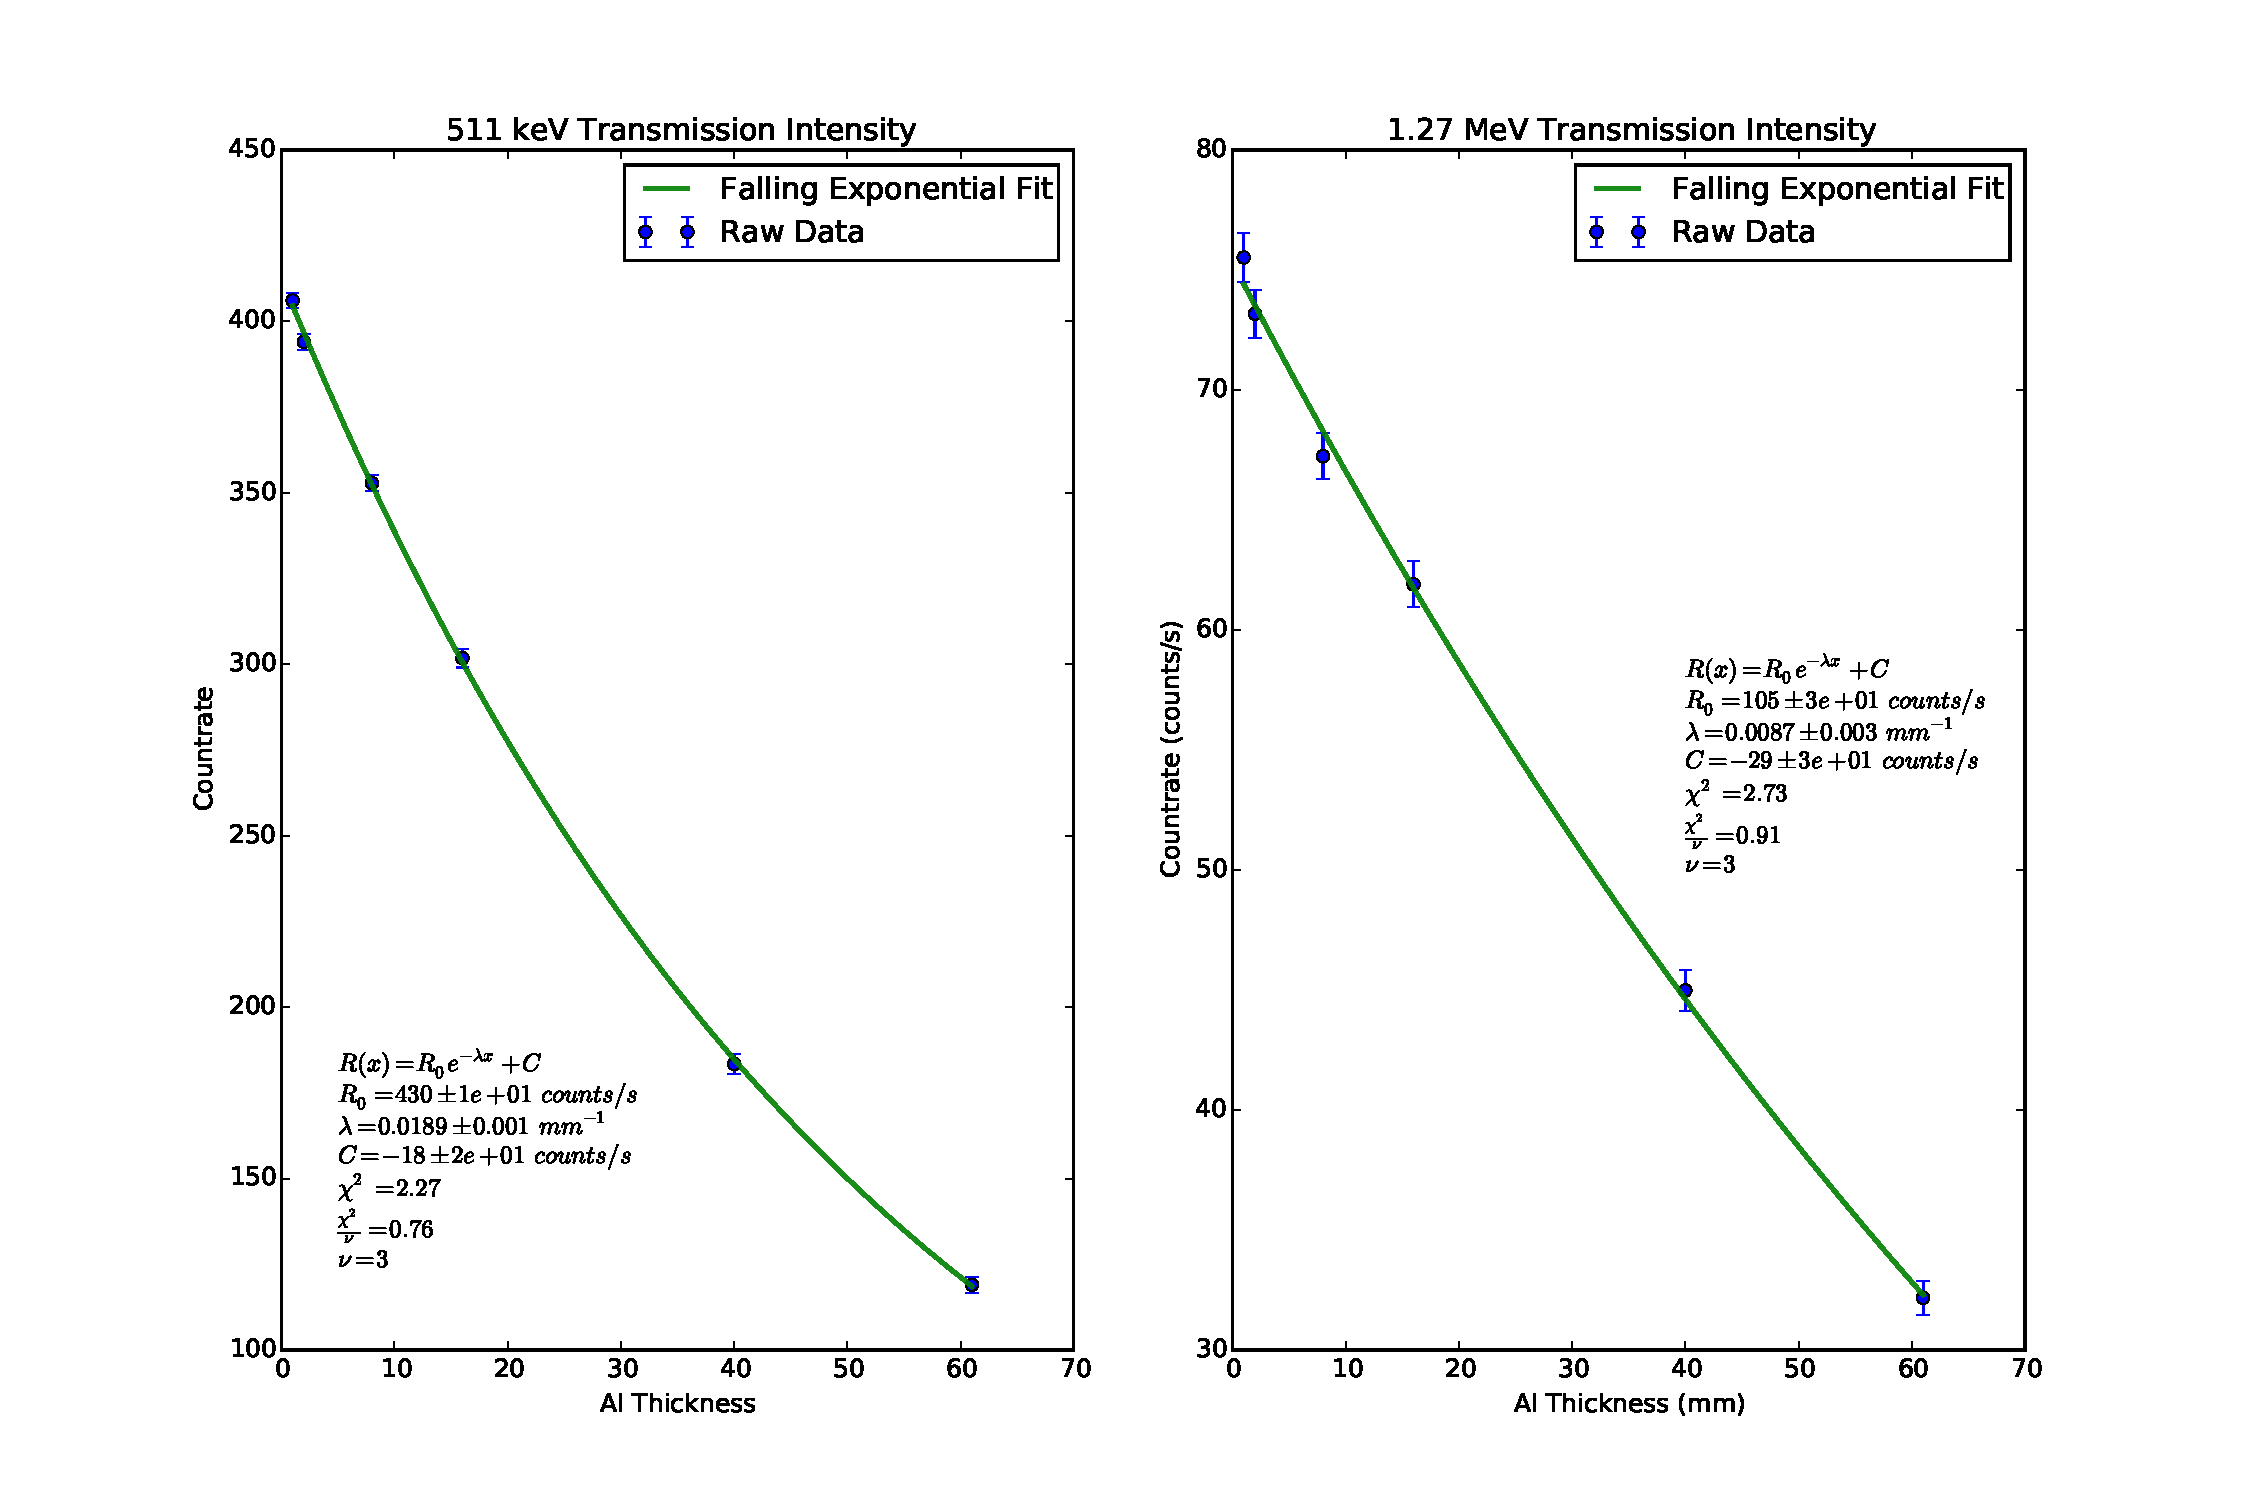
\includegraphics[scale=.5]{../plots/countrates_Na.pdf}
		\caption{The fit to the Na calculated countrates to obtain the linear attenuation coefficient, $\lambda$.  In order to convert from these values (in $mm^{-1}$) to the values in literature ($cm^{-1}$) simply multiply by 10.}
	\end{figure}
	\end{tightcenter}

	\begin{flushleft}
	The Na peaks fall in the region where the compton effect dominates, and our \redchi is less than 1 which indicates a good fit.  Therefore, the numbers we extract for $\lambda$ reflect our data well.  We tabulate fit-estimated values and uncertainty below.
	\end{flushleft}

	\begin{center}
	\begin{tabular}{|l|l|l|}
		\hline
		Energy & $\lambda$ & $\delta \lambda$\\ \hline
		511 keV & $0.19 \, cm^{-1}$ & $0.03 \, cm^{-1}$\\
		1.27 MeV & $0.09  \, cm^{-1}$ & $0.05 \, cm^{-1}$\\
		\hline
	\end{tabular}
	\end{center}

	\hspace{1cm}
	\subsubsection{Ba Countrates}

	The Ba peaks (fig. 6) fall more in the region where the photoelectric effect dominates, and so the fitting becomes more complicated.  A fit with a \redchi of approximately 167 (not shown) on the 31 keV peak tells us that the simple exponential fit is not sufficient.  By looking at the energy of this peak, we can deduce that the scattering is, while dominated by the photoelectric effect, not entirely compton-like or photoelectric-like.  Thus we update our fit model to take into account the data features more completely,
	\begin{equation}
		R(x) = R_0e^{-\lambda x} + R_0'e^{-\tau x} + C.
	\end{equation}
	This will tell us several important pieces of information: it will tell us approximately how much of this energy has the compton character and how much has the photoelectric character.  We use our $\lambda$ as the compton linear attenuation and $\tau$ as the photelectric linear attenuation.  Taking $\lambda + \tau$ should give us the total linear attenuation, which we can check against literature values.  We tabulate our values below.  The value for the 31 keV peak uncertainty we add in quadrature, making the assumption that the errors between $\lambda$ and $\tau$ are independent.  We make this assumption because upon inspection of the covariance matrix, the cross terms between $\lambda$ and $\tau$ are neglible - $\mathcal{O}(1e-10)$.  The other peaks did not fit this updated model well and so we keep the standard exponential form.

	\begin{center}
	\begin{tabular}{|l|l|l|}
		\hline
		Energy & $\lambda$ & $\delta \lambda$\\ \hline
		31 keV & $2.9 \, cm^{-1}$ & $0.1 \, cm^{-1}$\\
		81 keV & $0.513  \, cm^{-1}$ & $0.06 \, cm^{-1}$\\
		356 keV & $0.24 \, cm^{-1}$ & $0.04 \, cm^{-1}$\\
		\hline
	\end{tabular}
	\end{center}

	\begin{tightcenter}
	\begin{figure}[!htb]
		\centering
		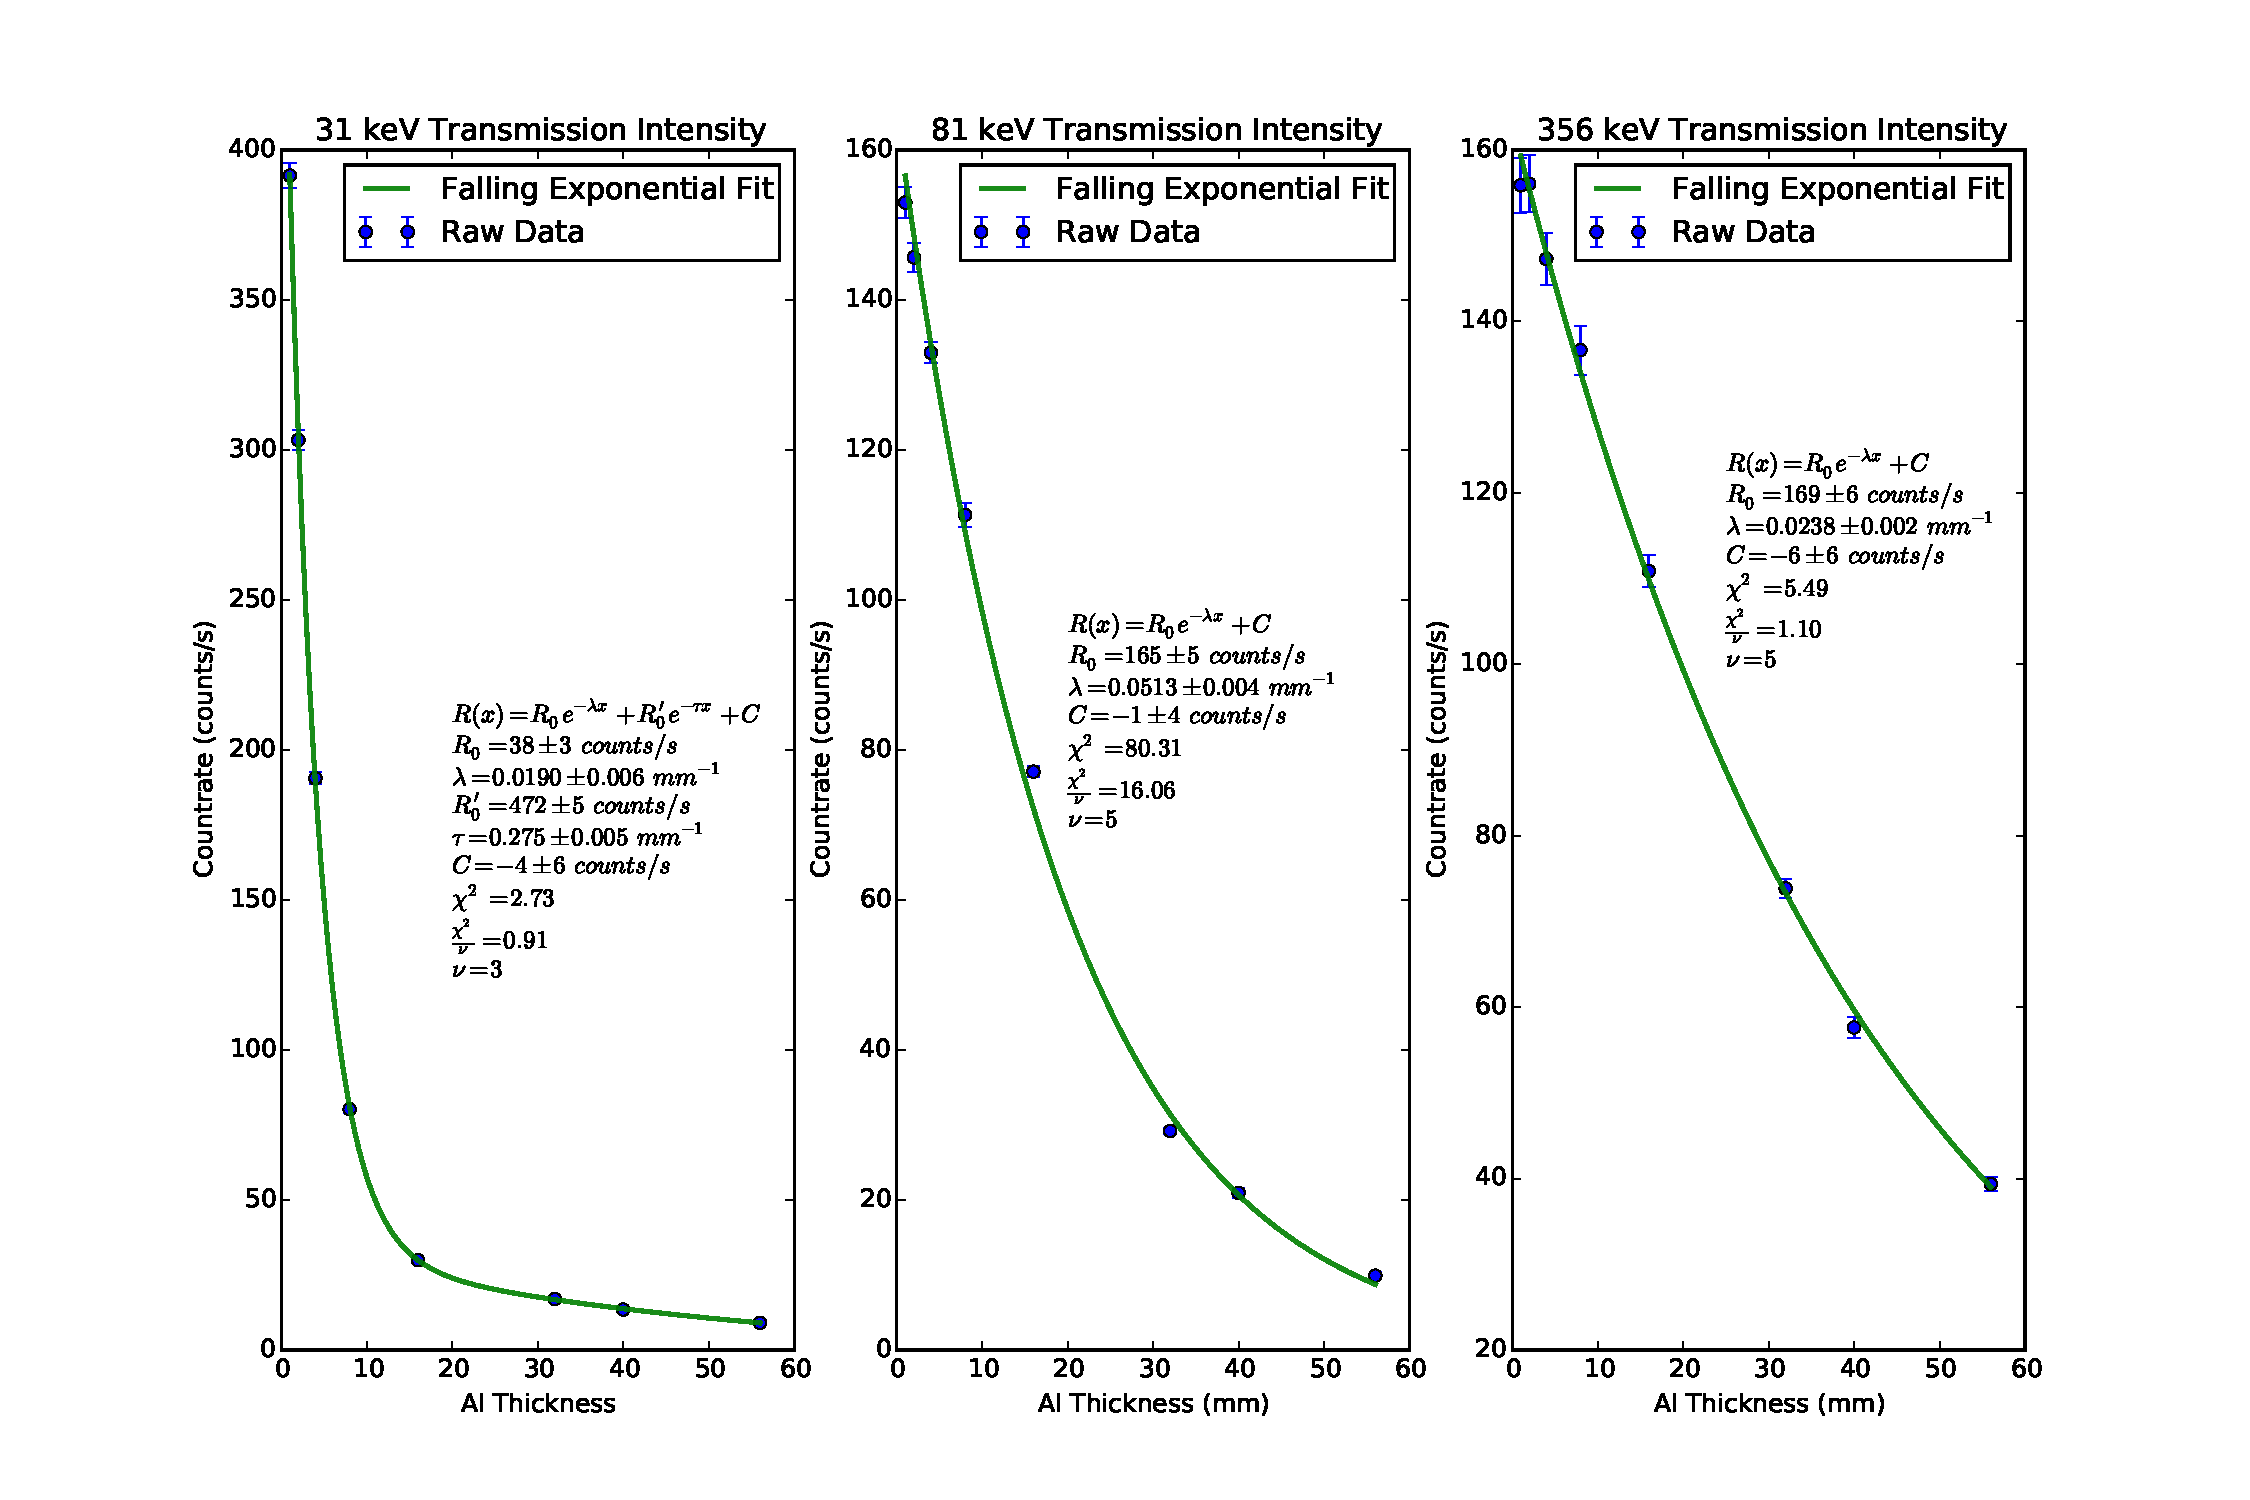
\includegraphics[scale=.5]{../plots/countrates_Ba.pdf}
		\caption{The fit to the Ba calculated countrates to obtain $\lambda$ and $\tau$, with $\lambda$ being the compton-like linear attenuation and $\tau$ being the photoelectric-like linear attenuation.  The total will just be $\lambda + \tau$.}
	\end{figure}
	\end{tightcenter}

	\subsubsection{Tabulating the Data}

	Now that we have all the values for $\lambda$ and the associated uncertainties, let's tabulate the values.  We will compare with values calculated from literature, and show our values plotted against those values.  The confidence levels are calculated the normal way, 
	\begin{gather*}
		t = \frac{\Delta}{\sigma_{\Delta}}\\
		C = 1-\erf\bigg{(}\frac{t}{\sqrt{2}}\bigg{)} \times 100\%
	\end{gather*}  
	These confidence levels are very conservative, the uncertainty in the calculated value is quite conservative.  These were based on values tabulated by NIST \cite{physics.nist.gov} whose energy levels were not quite what we measured but were within 10\% of the value.  We used for the uncertainty in those values an estimate based on the slope of the function that models $\lambda$ vs Energy at each point.  In one case (356 keV) we average the values tabulated by the NIST for 300 keV and 400 keV.  In the table below we have added our estimate for the systematic uncertainty in our values already.

	\begin{center}
	\begin{tabular}{|l|l|l|l|}
		\hline
		Energy & $\lambda \pm \delta \lambda  \, (cm^{-1})$ & $\lambda_{calc} \pm \delta\lambda_{calc}  (\, cm^{-1})$ & Confidence Level\\ \hline \hline
		31 keV & $2.9 \pm 0.1$ & $2.98 \pm 0.03$ & 57.6\%\\
		81 keV & $0.513 \pm 0.06$ & $0.533 \pm 0.03$ & 66.8\%\\
		356 keV & $0.24 \pm 0.04$ & $0.3 \pm 0.1$ & 79.0\%\\
		511 keV & $0.19 \pm 0.03$ & $0.22 \pm 0.05$ & 42.1\%\\
		1.27 MeV & $0.09 \pm 0.05$ & $0.15 \pm 0.07$ & 33.8\%\\
		\hline
	\end{tabular}
	\end{center}

	\begin{tightcenter}
	\begin{figure}[!htb]
		\centering
		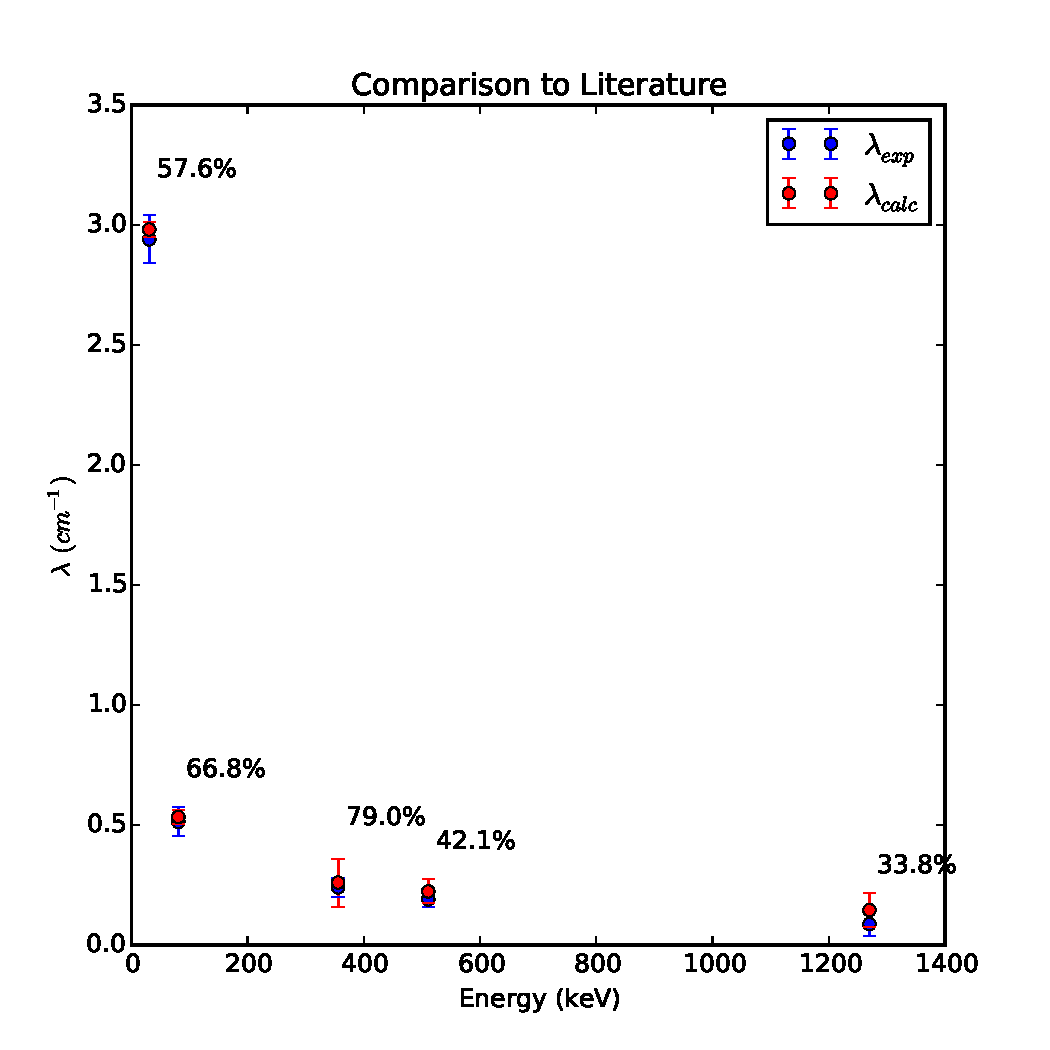
\includegraphics[scale=.5]{../plots/confidence}
		\caption{The confidence levels are shown above each datum.}
	\end{figure}
	\end{tightcenter}

\section{Error Analysis}
	\subsection{PHA Cross Sections}
	Since the errors in the Cross Sections portion of the experiment were of the variety that occur in counting, we use a simple $\sqrt{N}$ model for the uncertainty in the counts, which is reflected in the graph of the data (fig. 3, 4).  In propagating the uncertainty forward after performing the fits, we use the square root of the diagonal covariance matrix elements as the uncertainty in the fit parameters.  As was mentioned earlier, the largest uncertainty in the fit parameter for the net counts was approximately 3\%.

	\begin{flushleft}
	In the actual peak is encoded a width, broadening caused by the detector itself. That will be given by the Full Width at Half Maximum ($\Gamma$) of the fit.  It will be calculated by
	\end{flushleft}
	\begin{equation*}
		\Gamma = \sigma \sqrt{2}\sqrt{2i\pi + ln(2)}
	\end{equation*}
	which can be approximated as
	\begin{equation}
		\Gamma = \sigma \sqrt{2}\sqrt{ln(2)}.
	\end{equation}

	\begin{flushleft}
	We tabulate values of the energy and detector resolution, $\Gamma$, below.
	\end{flushleft}

	\begin{center}
	\begin{tabular}{|l|l|l|}
		\hline
		Energy (keV) & $\Gamma$ (channels) & $\Gamma/E$\\ \hline \hline
		31 & 8.36 & 26.9\%\\
		81 & 10.18 & 12.6\%\\
		356 & 30.25 & 8.49\%\\ \hline
		511 & 10.68 & 2.09\%\\
		1270 & 16.69 & 1.31\%\\
		\hline
	\end{tabular}
	\end{center}

	\begin{flushleft}
	At the line we switched from the Ba to the Na sample, and so the area in focus changed.  Furthermore we increased the gain by a factor of 4 (from 8 to 32) when taking data from the Ba-133 sample, which is very likely to have caused the decrease in detector resolution.
	\end{flushleft}

		\subsubsection{By Eye Estimation}
			Sometimes it can be useful to estimate parameters by eye.  We will choose the 356 keV peak on the Ba-133 spectrum, at an Aluminum thickness of 8mm to test our intuition for these values against the fitted values.  We will tabulate results below, as well as detail how to arrive at these values.

			\begin{gather*}
				\delta N = \sqrt{G + B}\\
				\sigma = \frac{\Gamma}{2\sqrt{ln(2)}}
			\end{gather*}

			\begin{center}
			\begin{tabular}{|l|l|l|}
				\hline
				Quantity & By Eye & Fitted\\ \hline \hline
				$N \pm \delta N (counts)$ & $27000 \pm 220$ & $33600 \pm 700$\\
				$\mu \pm \delta \mu$ & $670 \pm 5$ & $669.6 \pm 0.3$\\ 
				$\sigma \pm \delta \sigma$ & $35 \pm 6$ & $26.4 \pm 0.4$\\
				$\delta \mu  = \sigma/\sqrt{N}$ & $0.213$ & $0.144$\\
				\hline
			\end{tabular}
			\end{center}
			\begin{flushleft}
			The counts are notably different, while the others are quite similar.  The fit gives us smaller uncertainties in the parameters, though that assumes a good fit.  This particular peak has a \redchi = 1.55 and visually, it matches well.

			\vspace{.25cm}

			It is worth pondering why the counts are fairly different.  It seems as though the software overestimates the background, or the fit underestimates the background.  However, as we have seen from the countrates and further fitting to find the linear attenuation coefficient (which is the same as the literature value with a confidence level of 77.9\%) that use the fitted value, we are inclined to trust the fitted value.
			\end{flushleft}

	\subsection{Countrates}
	We calculated the countrates and fitted data generated by fitting the cross sections to gaussian models.  We assumed the standard uncertainty for a digital measurement device for time in computing the countrate - considering that the error in time of our shortest run was less than 0.001\%, we considered it to be negligible compared to the uncertainty in the fit parameter $N$.  Thus the error bars seen and the uncertainty in $\frac{N}{t}$ is simply
	\begin{equation}
		\sigma_{\dot{N}} = \sqrt{\cov(1,1)} \, ^{\dagger}.
	\end{equation}

	\begin{flushleft}
	$\tiny{^\dagger}$ It should be noted that in our fit, N was the first parameter - you would use whichever matrix element corresponds to N along the main diagonal.

	\vspace{.25cm}

	If we return momentarily to fig. 6, the 81 keV countrate fit, let us inspect for a moment the \redchi value.  It is unfortunately high.  This is likely to be caused by the fact that it is in the regime where the compton effect and the photoelectric effect are adding nearly at equal proportions.  We tried to fit it to the same model as the 31 keV rate, but that fit failed miserably.  Thus it is unlikely that a simple model will be able to describe the data perfectly.  However, we should not despair, as the fit still provides us with a value that matches the literature well.  Even if it did not, our other countrates still provide reliable sources of attenuation coefficients, and so we should not lose too much sleep over a single bad fit.
	\end{flushleft}

	\subsection{Systematic Uncertainties}
	After plotting our values for $\lambda$ and the values calculated from the NIST table, we see that all of our values are slightly lower.  This indicates some systematic error that needs to be accounted for.  A plausible explanation would include an exploration of the geometry of the apparatus - if the absorber disc is misplaced: too close or too far from the NaI crystal we will have a shifting of all the data up or down depending on if the Aluminum scatters the photons or accidentally redirects stray photons into the detector.  Thus there is an optimal length for the apparatus that we simply did not reach.  As discussed in the Apparatus section, we have added a 0.02 $cm^{-1}$ uncertainty to the value of each linear attenuation coefficient in order to take into account this systematic uncertainty.  This value is obtained by fitting the data and fitting the NIST data.  We fit to a model 
	\begin{equation*}
		f(x) = Ae^{Bx} + Ce^{Dx} + E.
	\end{equation*}
	This is far too complicated (and the fit is not shown to spare the reader's sensibilities), it was simply done as an attempt to find the systematic uncertainty present in our data.  Taking into account the uncertainty in each parameter, the difference between the fits was in the parameter E, and it was approximately $0.020 \pm 0.003$.  Thus we take this value (which simply shifts the entire function up or down) and use it as an estimate for our systematic uncertainty.

\section{Conclusion}
	We have concluded that fitting PHA cross sections is a very accurate way to determine counts, and by further fitting to determine the linear attenuation coefficient $\lambda$ we have found that measurement of these values can be done simply and with good precision.\\

	\begin{flushleft}
	This work was undertaken in cooperation with Mitch Spradlin.  We would like to thank the University of Chicago Advanced Undergraduate Laboratory faculty, staff and TAs for their help and willingness to answer inane questions about obscure subjects.
	\end{flushleft}

\begin{thebibliography}{10}
	\bibitem{physics.nist.gov}
		Seltzer, et al. "X-Ray Mass Attenuation Coefficients" NIST.\\
		http://physics.nist.gov/PhysRefData/XrayMassCoef/ElemTab/z13.html. (Accessed Oct 16, 2015)
	\bibitem{lab manual}
		University of Chicago Department of Physics. "Introductory Lab: Gamma Cross Sections"\\
		https://wiki.uchicago.edu/display/P211manuals/Introductory+Lab\%3A+Gamma+Cross+Sections. (Accessed Oct 8-16, 2015)

	\bibitem{taylor}
		Taylor, John. \emph{An Introduction to Error Analysis}. Sausalito: University Science Books, 1997.
	\bibitem{sample}
		Baumer, Michael. \emph{Gamma Cross Sections}.  University of Chicago Physics Department, Advanced Sample Lab Report.
\end{thebibliography}



\end{document}